\begin{frame}{}
  \begin{block}{}
	In 1982, Conway and others showed Life can simulate:
	\begin{itemize}
	\item memory cells
	\item wires
	\item a clock
	\item logic gates
	\end{itemize}
  \end{block}
  \begin{block}{}
	In 2000, Rendell implemented a Turing Machine in Life, and extended it to a
	universal Turing Machine in 2010.
  \end{block}
\end{frame}

\begin{frame}{Basic concepts for the construction}
  \begin{columns}
	\begin{column}{0.5\textwidth}
	  \begin{itemize}
	  \item gliders transmit information
	  \item a glider's presence = 1, absence = 0
	  \item glider guns repeatedly create gliders
	  \item collide gliders to compute with data
	  \end{itemize}
	\end{column}
	\begin{column}{0.49\textwidth}
	  \animategraphics[loop,autoplay,width=\textwidth]{10}{glider-gun-}{0}{29}
	\end{column}
  \end{columns}
\end{frame}

\begin{frame}{Memory cells}
  \begin{columns}
	\begin{column}{0.5\textwidth}
	  \begin{itemize}
	  \item information stored in circling gliders
	  \item gliders duplicated when we wish to read stored value
	  \item read is triggered by gliders hitting pentadecathlon at top right
	  \end{itemize}
	\end{column}
	\begin{column}{0.5\textwidth}
	  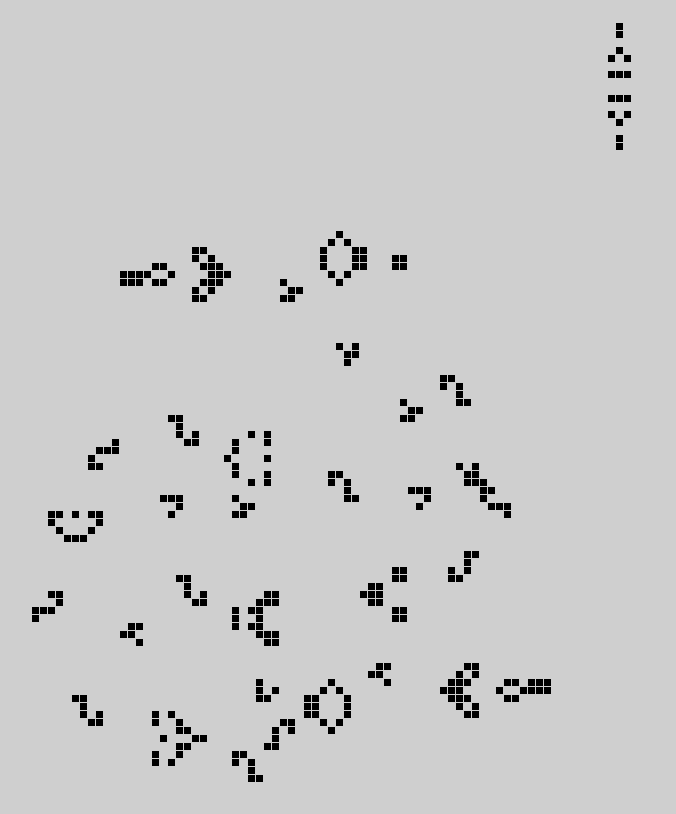
\includegraphics[width=\textwidth]{memory-cell}
	\end{column}
  \end{columns}
\end{frame}

\begin{frame}{The transition function}
  \begin{columns}
	\begin{column}{0.5\textwidth}
	  \begin{itemize}
	  \item grid of memory cells
	  \item rows indexed by state, columns indexed by symbol
	  \item each memory cell contains enough information for a transition: new
		state, new symbol and motion
	  \end{itemize}
	\end{column}
	\begin{column}{0.5\textwidth}
	  \centering
	  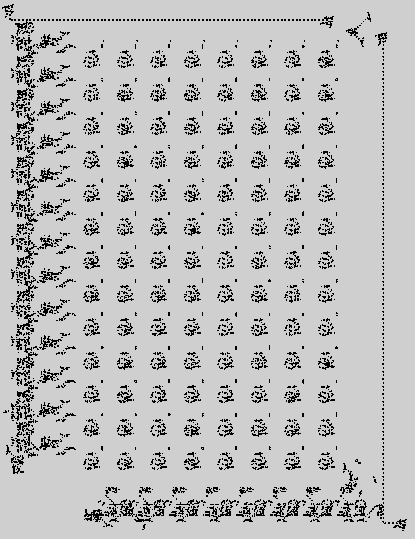
\includegraphics[width=0.92\textwidth]{transition-function}
	\end{column}
  \end{columns}
\end{frame}

\begin{frame}{The tape}
  \begin{columns}
	\begin{column}{0.5\textwidth}
	  \begin{itemize}
	  \item two stacks instead of a tape
	  \item tape motion is performed by a pop and push operation
	  \item no memory cell for symbol at current head position
	  \end{itemize}
	\end{column}
	\begin{column}{0.5\textwidth}
	  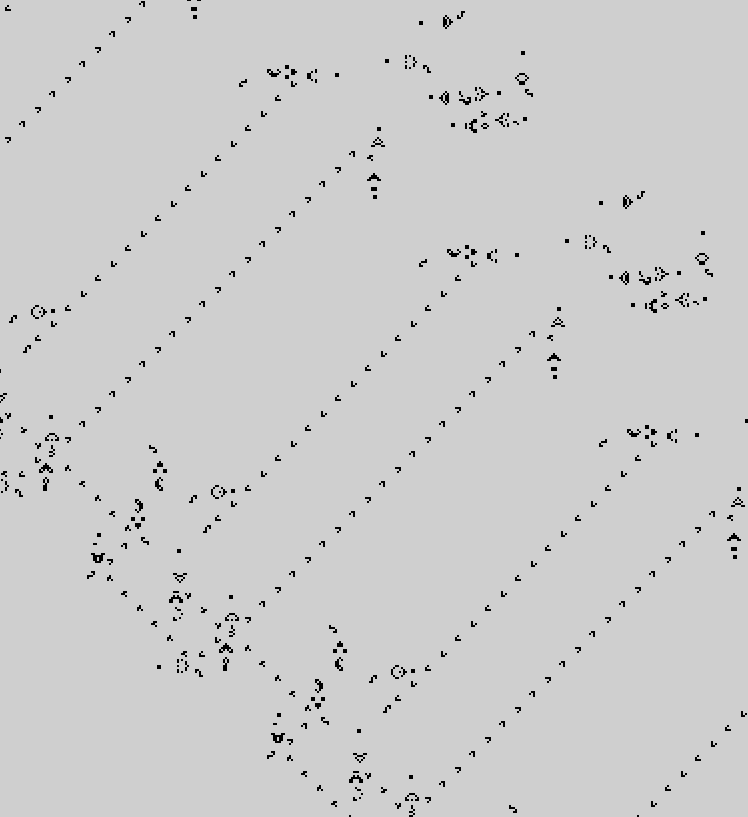
\includegraphics[width=\textwidth]{tape}
	\end{column}
  \end{columns}
\end{frame}

\begin{frame}{The full Turing machine}
  \centering
  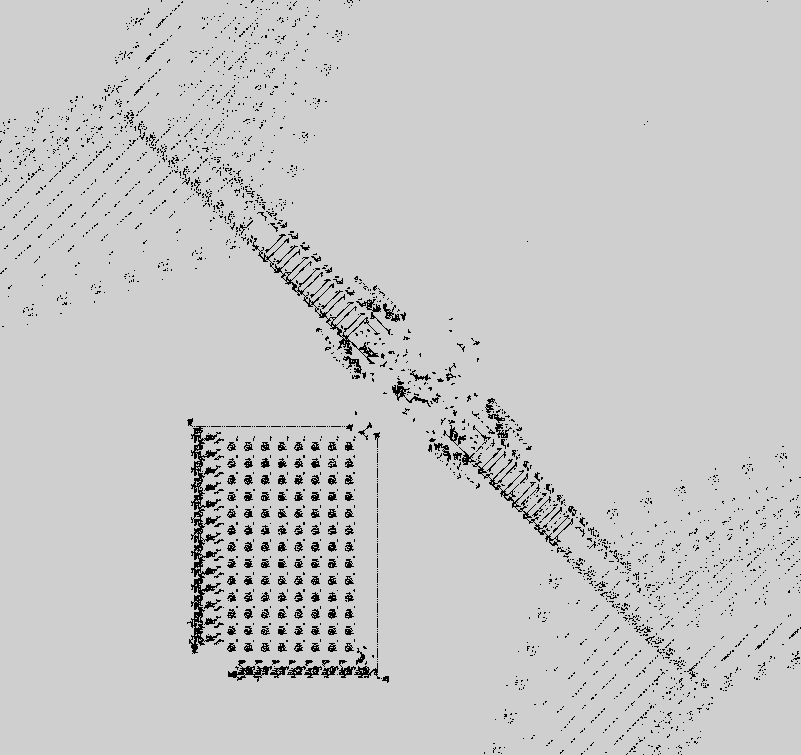
\includegraphics[width=0.6\textwidth]{full}
\end{frame}